\documentclass{beamer}
\mode<presentation>
{
  \usetheme{Boadilla}      % or try Darmstadt, Madrid, Warsaw, ...
  \usecolortheme{default} % or try albatross, beaver, crane, ...
  \usefonttheme{default}  % or try serif, structurebold, ...
  \setbeamertemplate{navigation symbols}{}
  \setbeamertemplate{caption}[numbered]
  \setbeamerfont{caption}{size=\scriptsize}
  \setbeamercolor{alerted text}{fg=blue}
} 

\usepackage[english]{babel}
\usepackage[utf8x]{inputenc}
\usepackage{hyperref}
\usepackage{comment}
\usepackage[natbibapa]{apacite} % Bibliography management
\usepackage{pdfpages}

\title[Open access workshop]{Open Access: Background and Tools for Early Career Researchers in Social Sciences}
\subtitle{Workshop prepared for the Berlin Summer School in Social Sciences}
\author[P. Joly]{Philippe Joly}
\institute[HU-Berlin \& WZB]{\texttt{\href{mailto:jolyphil@hu-berlin.de}{jolyphil@hu-berlin.de}} \newline Humboldt-Universität zu Berlin \newline \& \newline WZB Berlin Social Science Center}
\date{18 July 2018}

\begin{document}

%------------------------------------------------------------------

\begin{frame}
  \titlepage
\end{frame}

%------------------------------------------------------------------

\begin{frame}{}
	\footnotesize{
    \includegraphics[width=0.2\textwidth]{ccby.eps}
    
    ---
    
    \textbf{Reuse of the material}

The contents of the workshop are under a \href{https://creativecommons.org/licenses/by/4.0/}{CC BY 4.0} license, except when specified differently in the legend of certain figures.

	All the material of this workshop (the outline, the slides, and the bibliography) can be cloned or downloaded from GitHub:

	\href{https://github.com/jolyphil/oa-workshop}{https://github.com/jolyphil/oa-workshop}

	---

	\textbf{Acknowledgements}
    
    This workshop was prepared as part of the  \href{https://www.wikimedia.de/wiki/Fellowprogramm}{Freies Wissen Fellowship} sponsored by Wikimedia Deutschland, the Stifterverband, and the VolkswagenStiftung. It largely benefited from the webinar on open access presented by Christina Riesenweber (FU-CeDiS) and Agnieszka Wenninger (FU-CeDiS) on January 31, 2018, as part of the Freies Wissen Fellowship. Part of the references were found on the Open Science MOOC. Alessandro Blasetti (WZB) provided useful resources on OA licenses.
	}
\end{frame}

%------------------------------------------------------------------

\begin{frame}{}
\begin{figure}
	
\includegraphics[width=0.5\textwidth]{fellow.png}
        \caption{Logo of the Fellowship ``Freies Wissen''. Source: \citet{wikimedia_deutschland_fellow-programm_2018}. License: \href{CC BY-SA 3.0}{CC BY-SA 3.0}.}
\end{figure}
\end{frame}

%------------------------------------------------------------------

\begin{frame}{Overview}
	\begin{itemize}
    	\uncover<1->{
        \item Objectives
        }
        \begin{enumerate}
        	\uncover<2->{
        	\item Give early career researchers in social sciences a \textbf{basic knowledge} of open access (focus: papers).
            }
            \uncover<3->{
             \item Present useful \textbf{tools}.
             }
        \end{enumerate}
        \uncover<4->{
        \item Structure
        \begin{enumerate}
        	\item What is wrong with the subscription-based publication system?
            \item What is open access publishing?
            \item \textit{Discussion}
            \item What is the share of open access publications and what is their impact?
            \item Which license should you choose?
            \item How to find funding for your open access publication?
            \item \textit{Practical examples}
            \item \textit{Q\&A}
        \end{enumerate}
         }
	\end{itemize}
\end{frame}

%------------------------------------------------------------------

\begin{frame}{}
\begin{figure}
	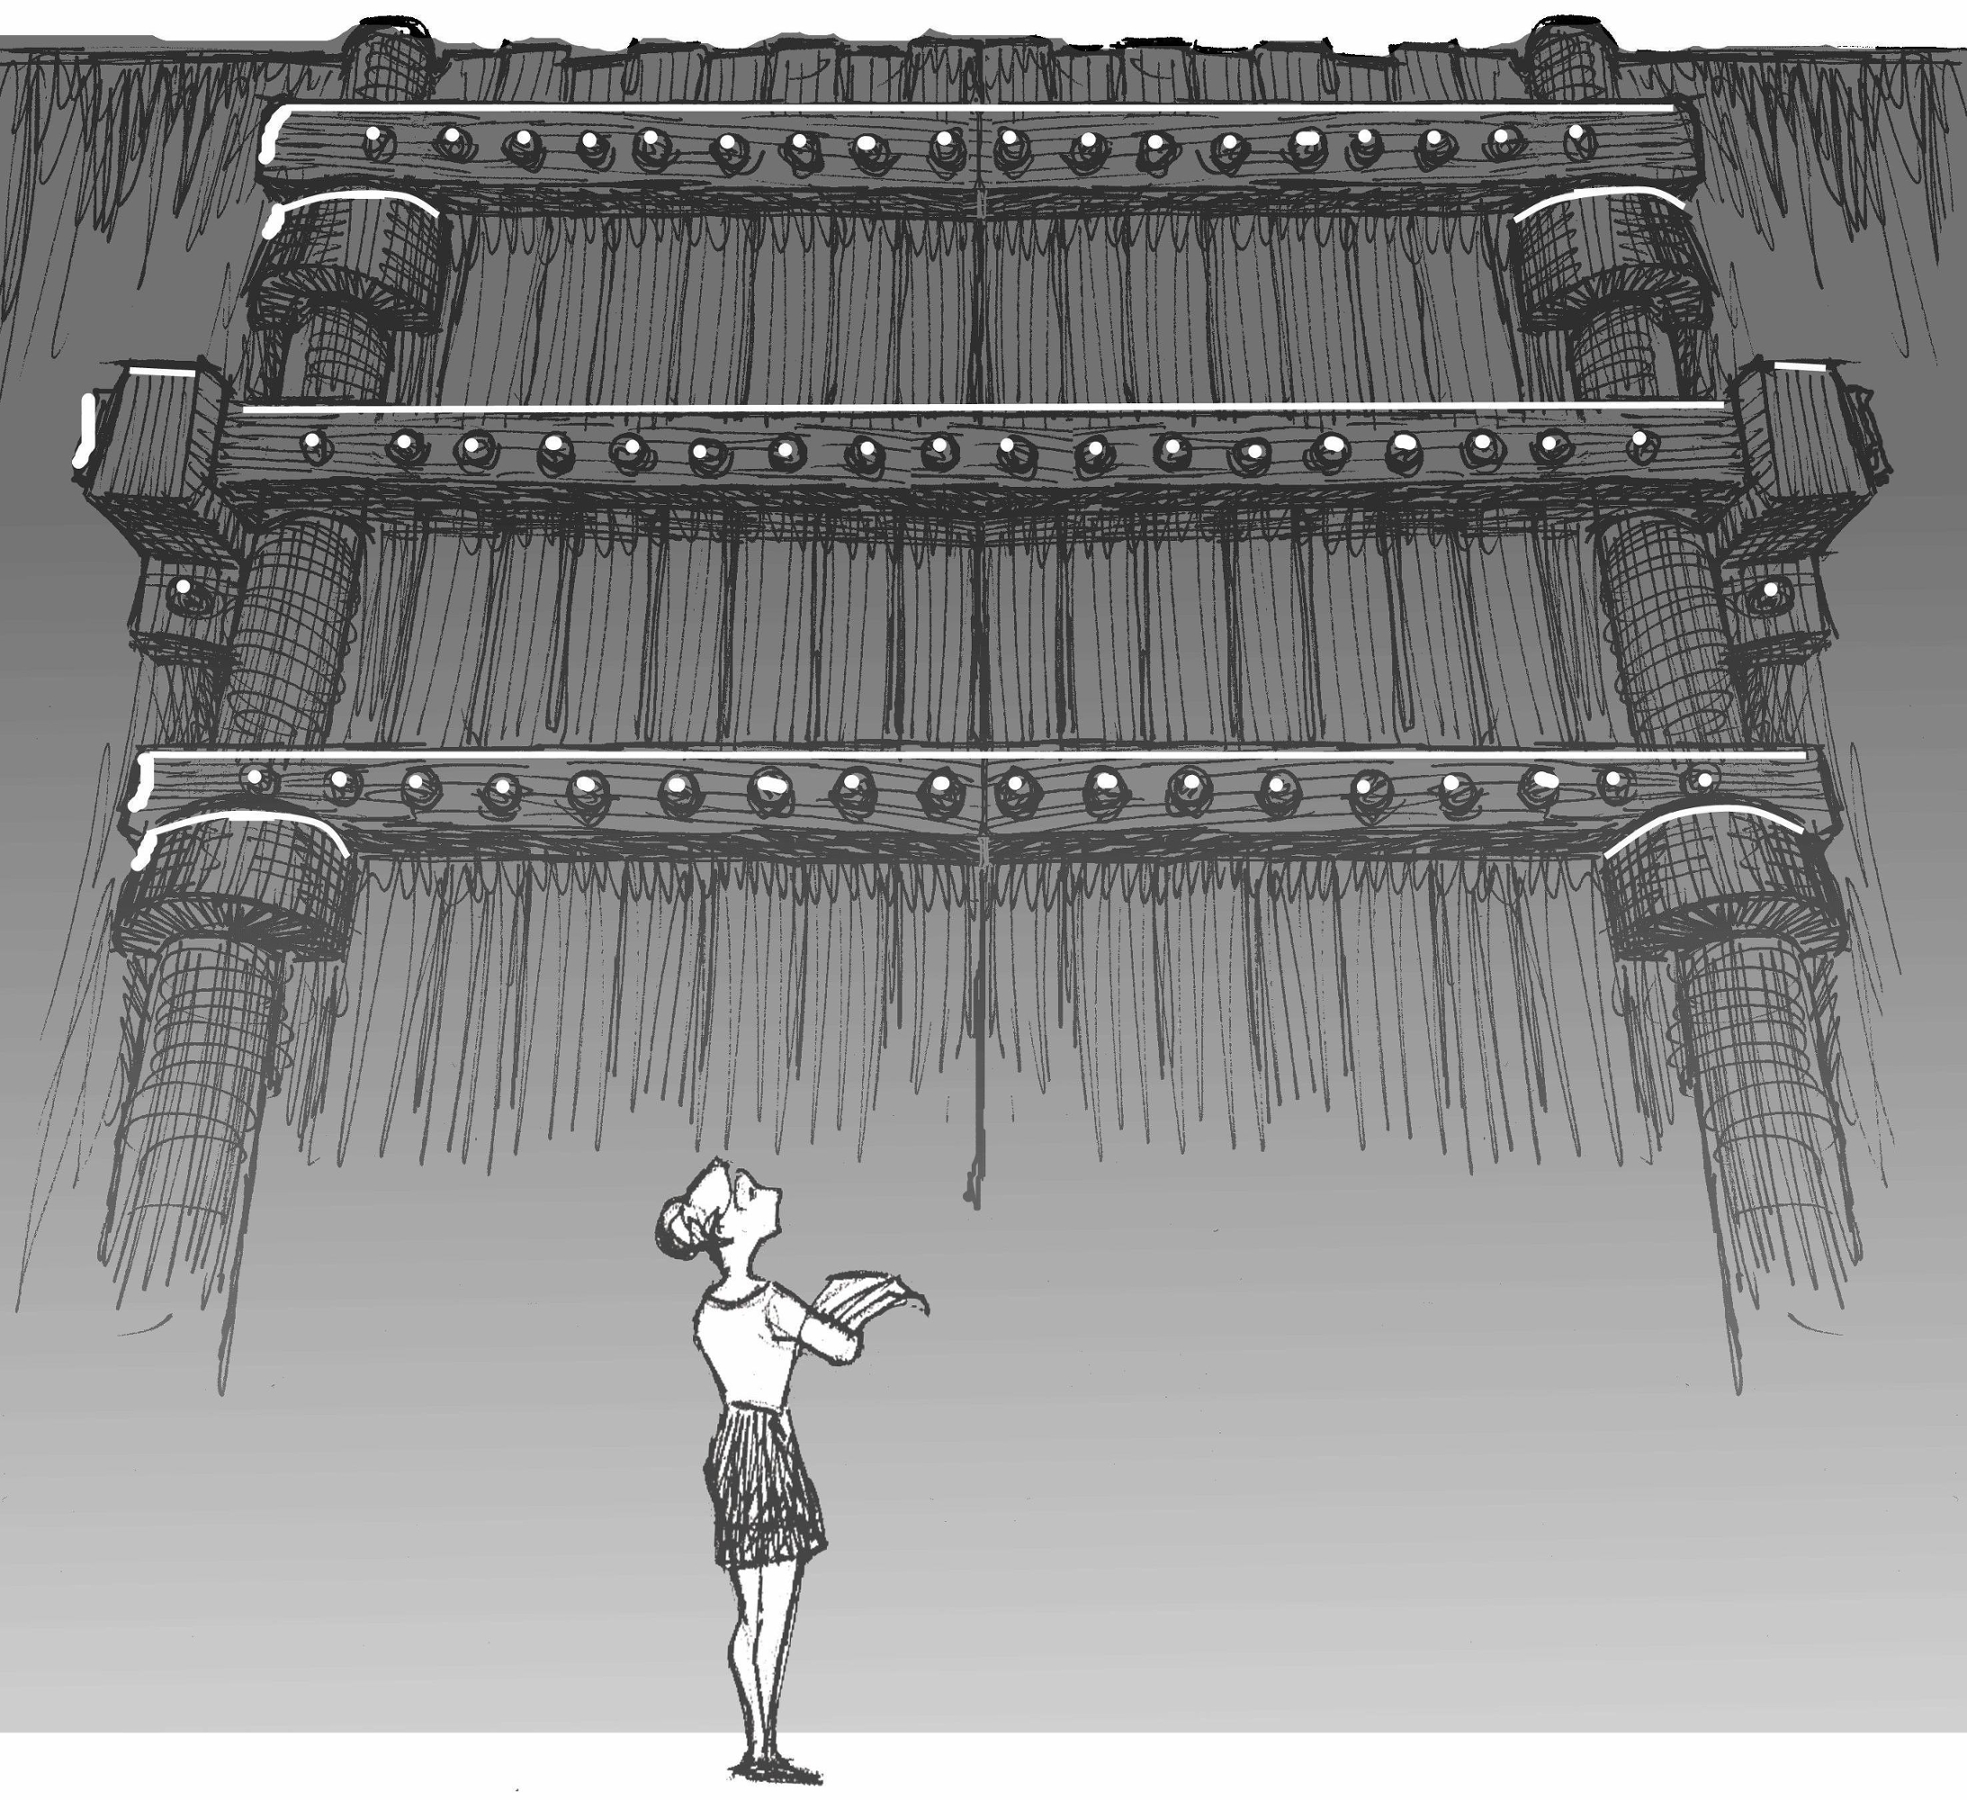
\includegraphics[width=0.5\textwidth]{mckiernan_1.jpg}
	\caption{Scientific information is locked behind paywalls. Source: John R. McKiernan from the \citet{why_open_research?_image_nodate} project. License: \href{https://creativecommons.org/licenses/by/4.0/}{CC BY 4.0}.}
\end{figure}
\begin{center}
	\textbf{\large What is wrong with the subscription-based system?}
\end{center}
\end{frame}

%------------------------------------------------------------------

\begin{frame}{Background}
	\begin{itemize}
    	\uncover<1->{
    	\item Journal articles are one of the oldest ways of communicating research results (350 years).
        }
        \uncover<2->{
        \item For long, journals were mostly managed by academic societies.
        }
        \uncover<3->{
        \item But there was a turn after the Second World War:
        }
        \begin{enumerate}
        	\uncover<4->{
        	\item More \textbf{specialization} and an \textbf{increase in the number of journals}.
            }
            \uncover<5->{
            \item Creation and \textbf{acquisition} of journals by commercial publishers.
            }
            \uncover<6->{
            \item Adoption of \textbf{impact factors} as main metric of scientific achievement. 
            }
            \uncover<7->{
            \item Commercial publishers secure their hold on \textbf{``A'' journals} \citep{buranyi_is_2017}.
            }
        \end{enumerate}
	\end{itemize}
\end{frame}

%------------------------------------------------------------------

\begin{frame}{The digital turn and the consolidation of the Big Five}
	\begin{itemize}
    	\uncover<1->{
    	\item Things got \textbf{worse} in the digital era \citep{lariviere_oligopoly_2015}.
        }
        \uncover<2->{
        \item Acquisitions of small journals continued.
        }
        \uncover<3->{
        \item This led to the consolidation of the \textbf{``Big Five:''}
        \begin{enumerate}
        	\item Elsevier
            \item Wiley-Blackwell
            \item Springer
            \item Taylor \& Francis
            \item Sage
        \end{enumerate}
        }
	\end{itemize}
\end{frame}

%------------------------------------------------------------------

\begin{frame}{``Big deals''}
	\begin{itemize}
    	\uncover<1->{
    	\item Libraries stop subscribing to individual journals.
        }
        \uncover<2->{
        \item They subscribe to entire online catalogs.
        }
        \uncover<3->{
        \item ``Big deals'' mean almost zero marginal costs for publishers.
        }
        \uncover<4->{
        \item Libraries become a captive market, prices skyrocket.
        }
        \uncover<5->{
        \item The Big Five now publish \textbf{50\%} of all scientific papers each year \citep{lariviere_oligopoly_2015}.
        }
	\end{itemize}
\end{frame}

%------------------------------------------------------------------

\begin{frame}{The Big Five in social sciences and humanities}
	\begin{figure}
		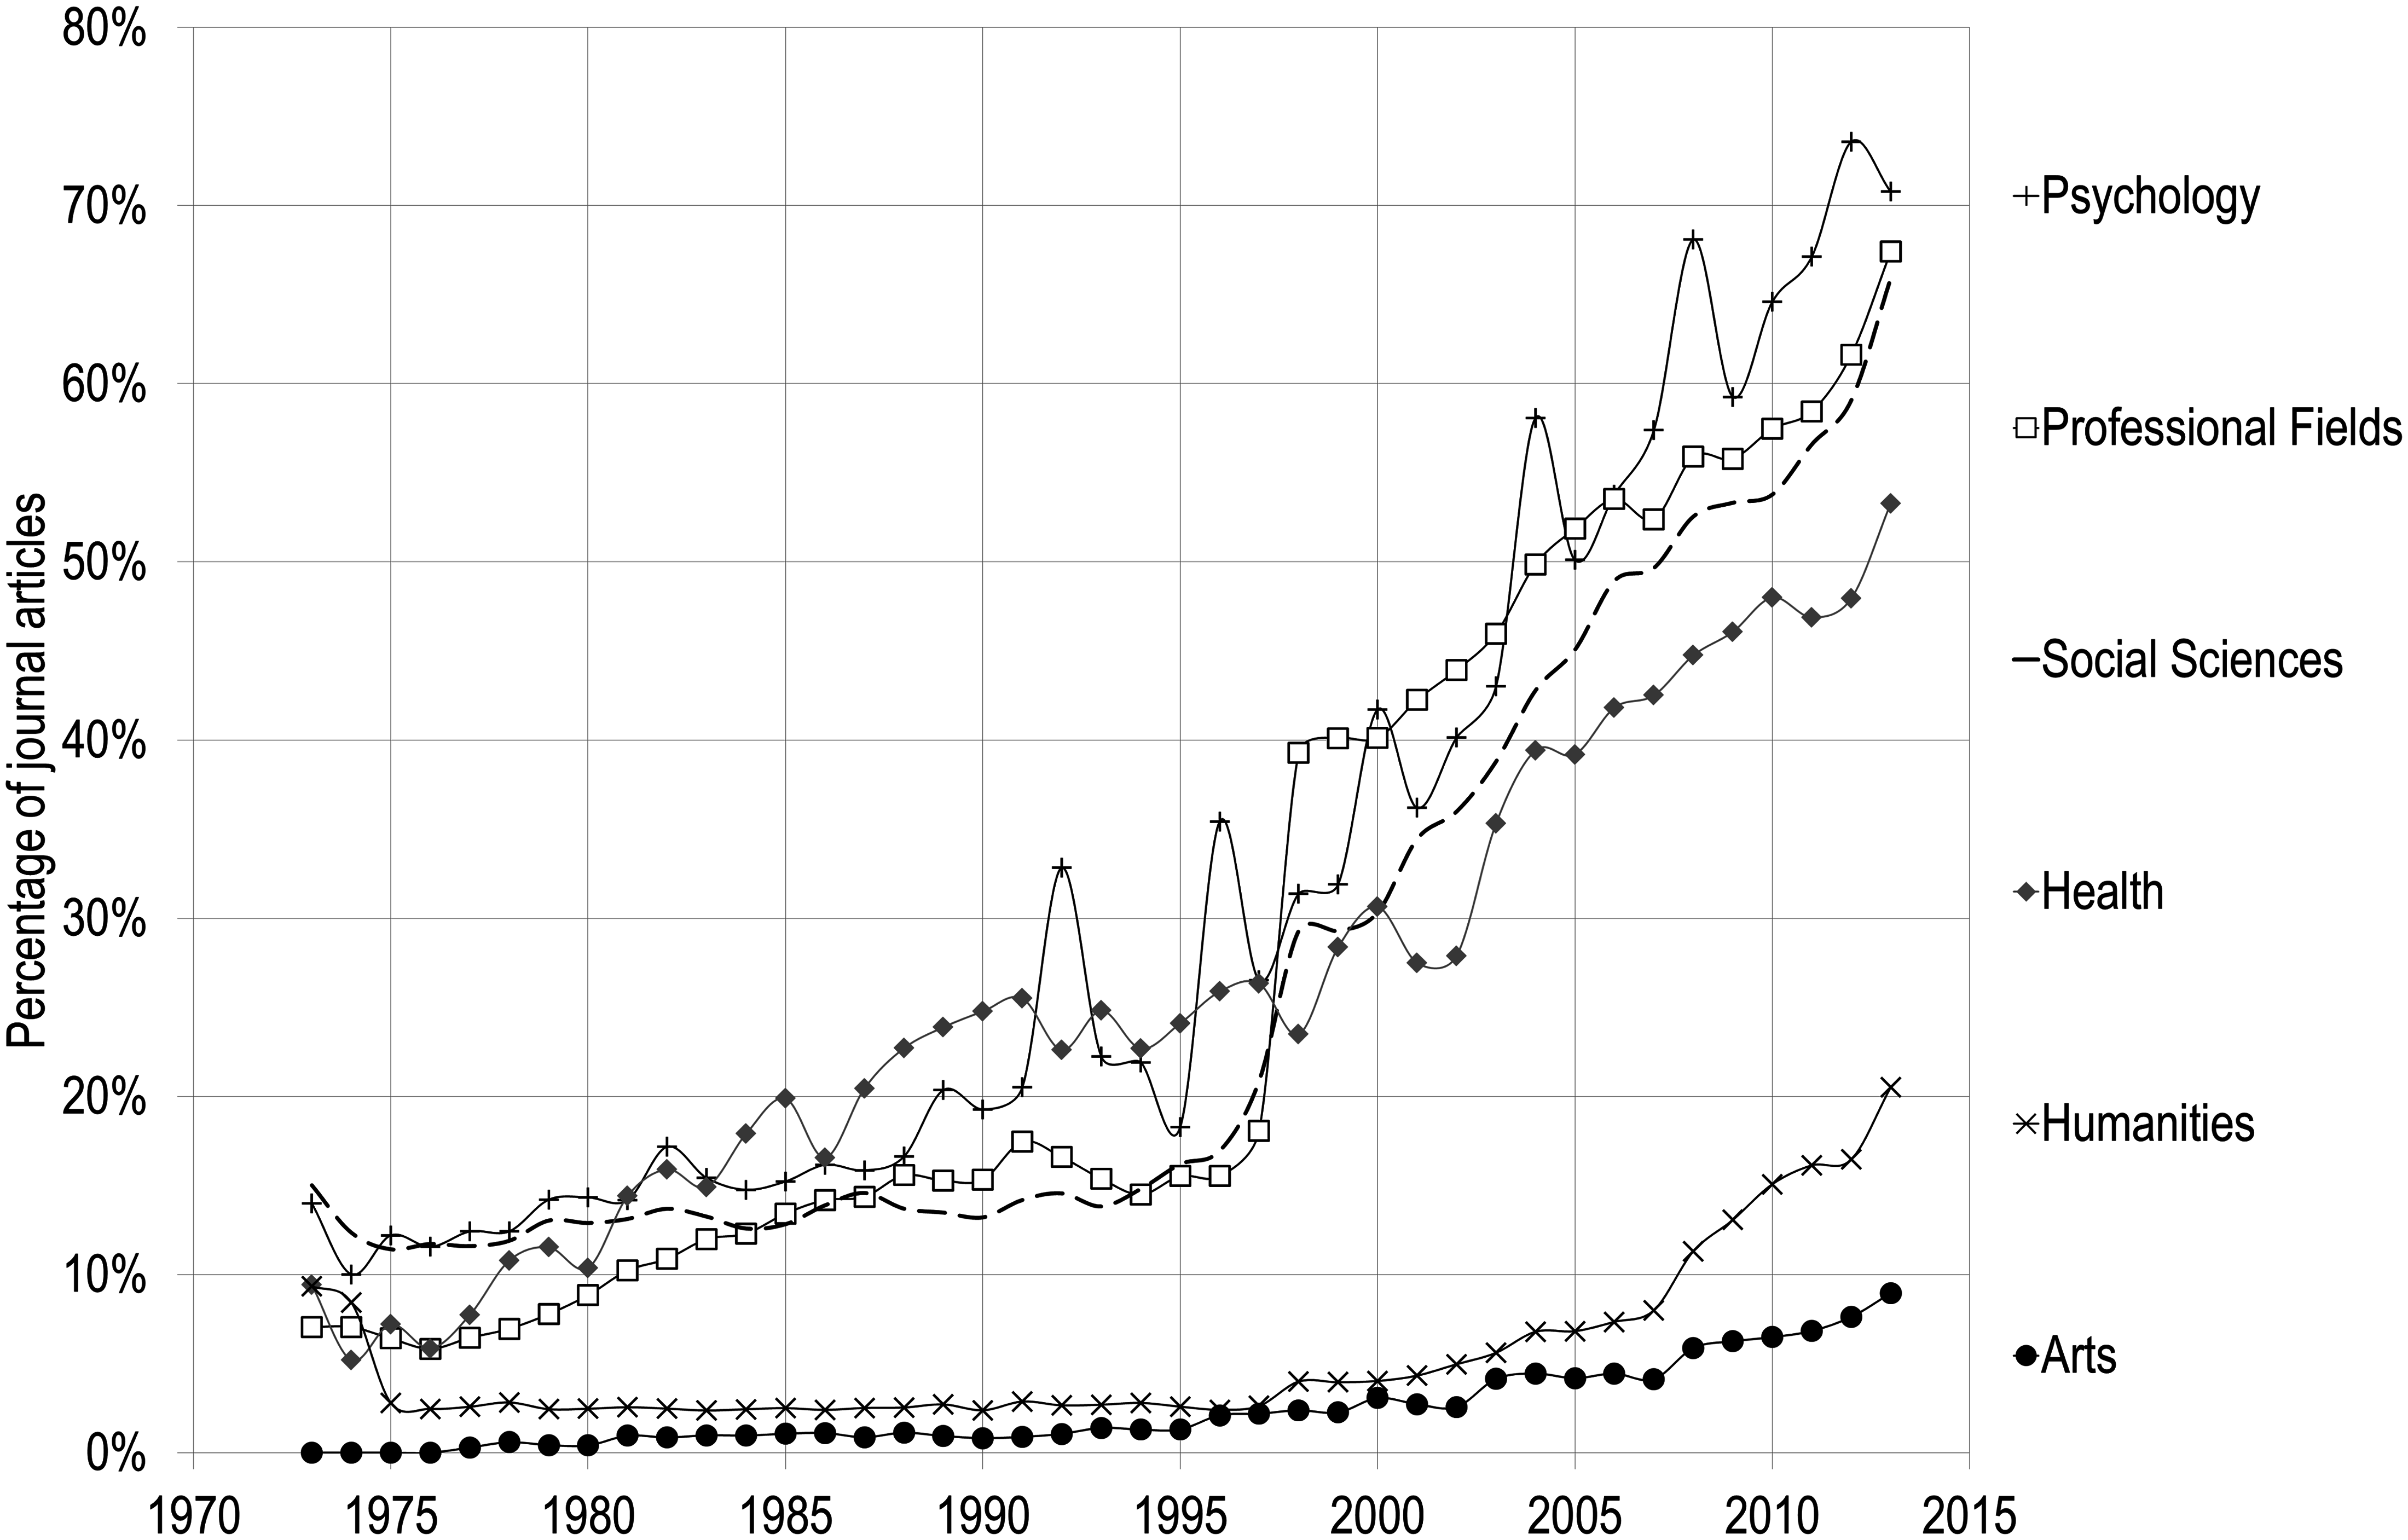
\includegraphics[width=0.9\textwidth]{lhm_1.png}
		\caption{Percentage of papers published by the five major publishers, by discipline of social sciences and humanities. Source: \citet{lariviere_oligopoly_2015}. License: \href{https://creativecommons.org/licenses/by/4.0/}{CC BY 4.0}.}
	\end{figure}
\end{frame}

%------------------------------------------------------------------

\begin{frame}{The trap}
	\begin{itemize}
    	\uncover<1->{
    	\item The current publishing system is a \textbf{system of exploitation}.
        }
        \uncover<2->{
        \item Most of the work is carried out \textbf{for free} by authors and reviewers.
        }
        \uncover<3->{
        \item There is no competition in the academic publishing sector.
        }
        \uncover<4->{
        \item Publishers have tremendous power over the access to knowledge.
        }
        \uncover<5->{
        \item Publishers are big enough to impose their conditions (e.g. Elsevier: \textbf{25\%} of the entire scientific literature).
        }
	\end{itemize}
\end{frame}

%------------------------------------------------------------------

\begin{frame}{An extremely lucrative business}
\begin{figure}
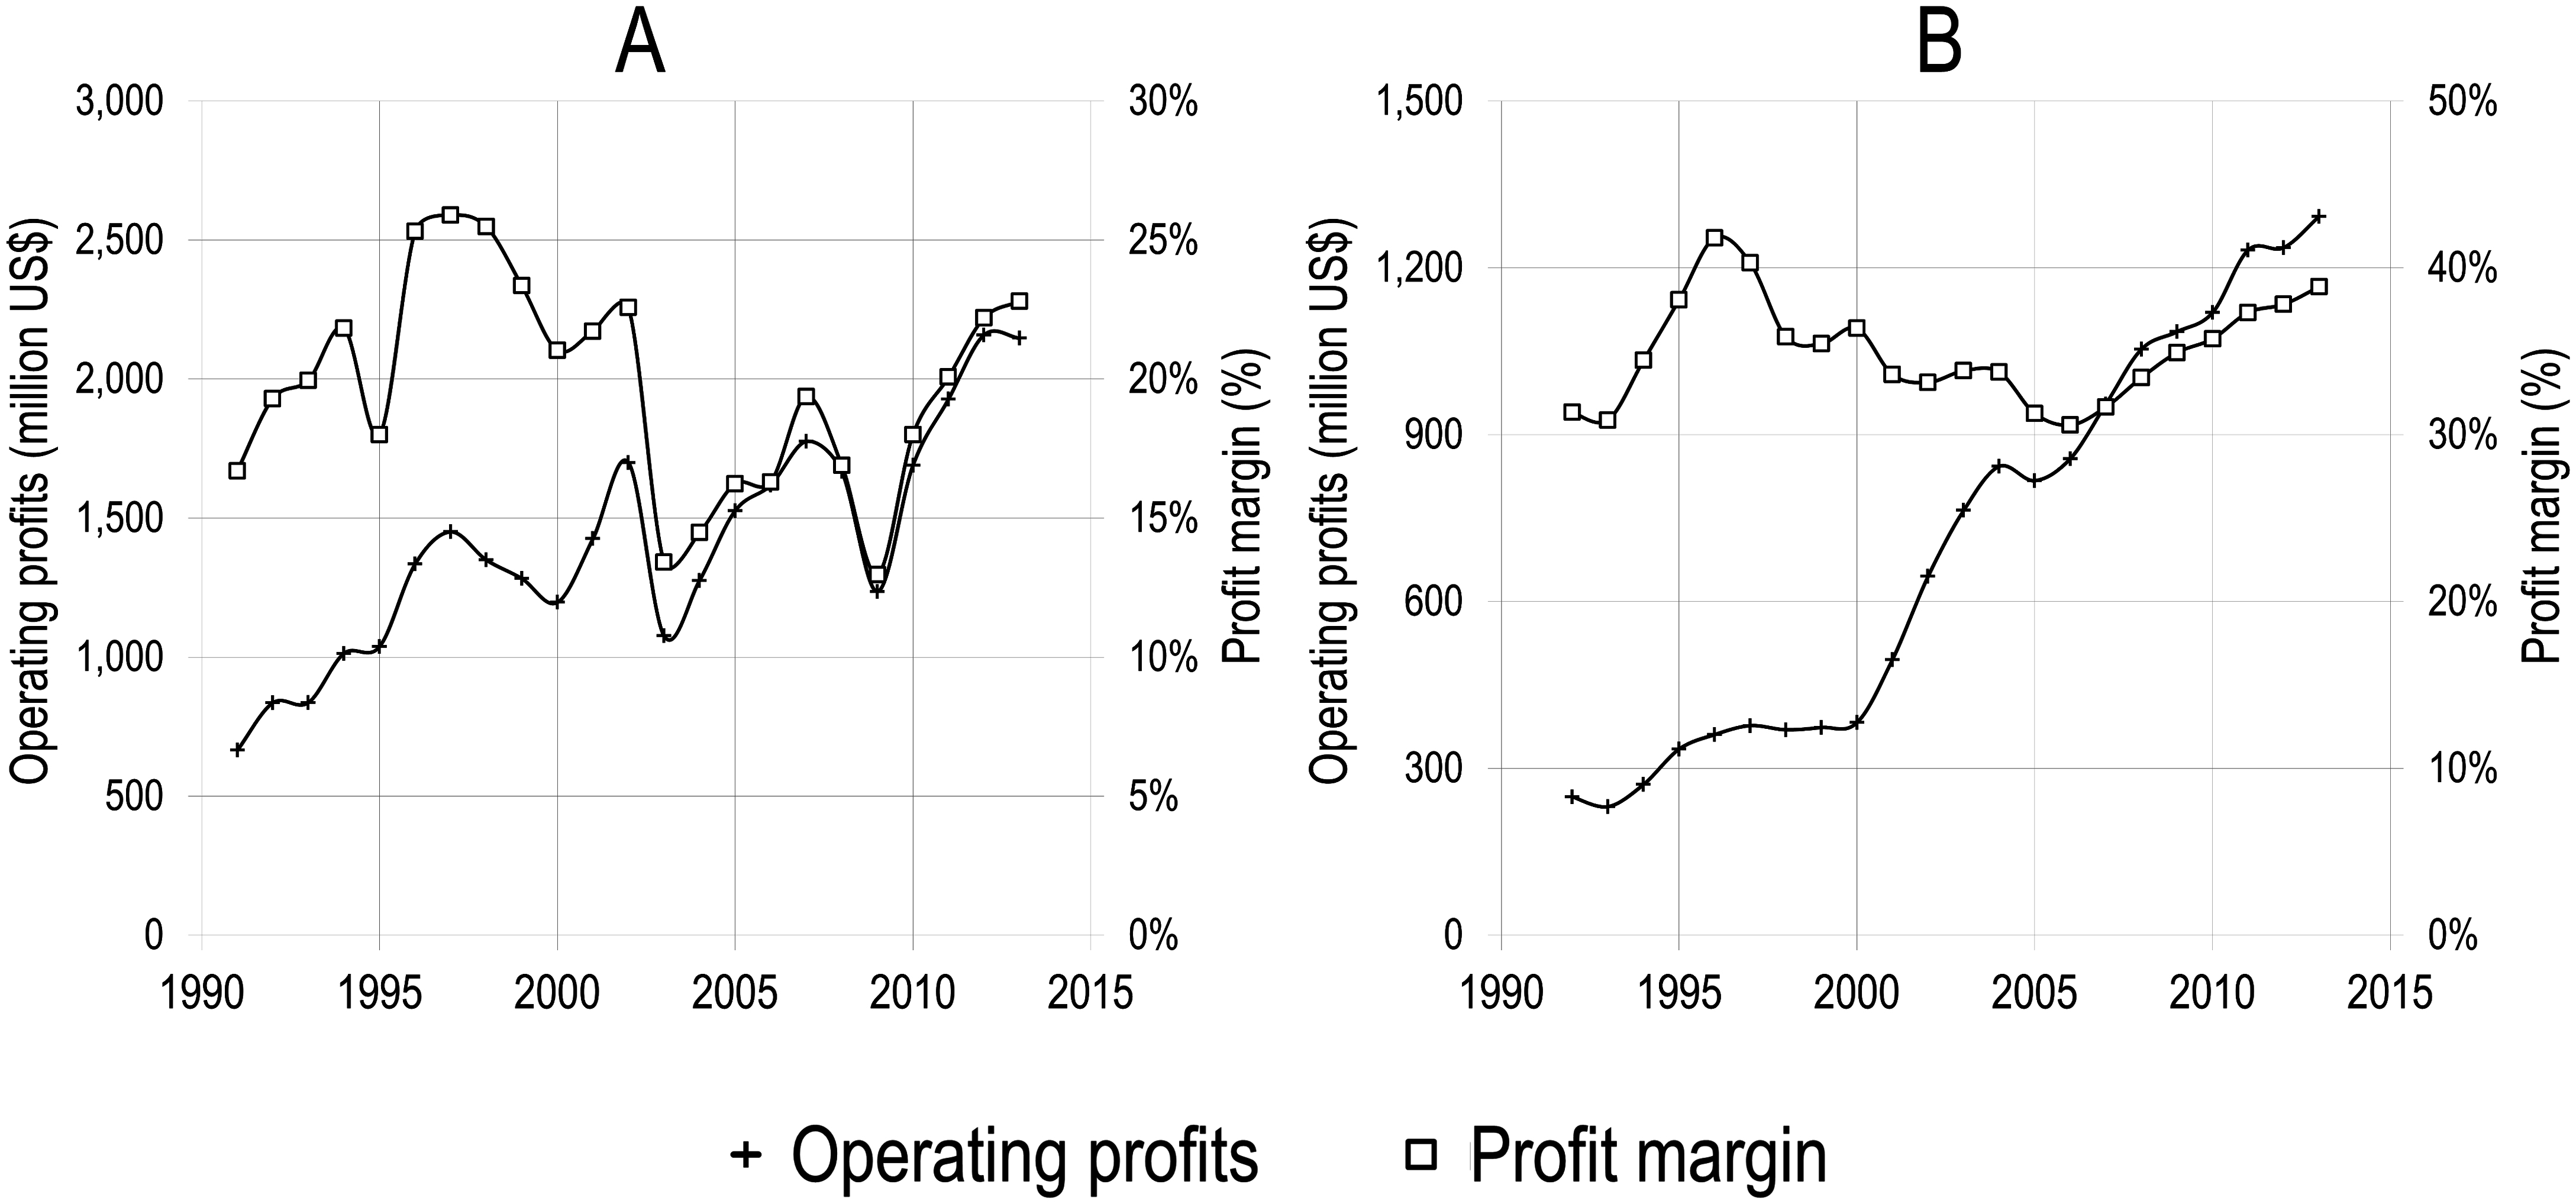
\includegraphics[width=\textwidth]{lhm_2.png}
\caption{Operating profits (million USD) and profit margin of Reed-Elsevier as a whole (A) and of its Scientific, Technical \& Medical division (B), 1991-2013. Source: \citet{lariviere_oligopoly_2015}. License: \href{https://creativecommons.org/licenses/by/4.0/}{CC BY 4.0}.}
\end{figure}
\end{frame}

%------------------------------------------------------------------

\begin{frame}{Consequences}
	\begin{itemize}
    	\uncover<1->{
    	\item Governments (the public) pay twice for research and access to the literature.
        }
        \uncover<2->{
        \item Libraries are no more capable of affording the publishers' ``big deals.''
        }
        \uncover<3->{
        \item With cancellations, students and researchers loose access to large portions of the scientific literature. 
        }
        \uncover<4->{
        \item The public and institutions with less funding (especially in low- and middle-income countries) are kept in the dark.
        }
	\end{itemize}
\end{frame}

%------------------------------------------------------------------
% 2. What is Open Access Publishing?
%------------------------------------------------------------------

\begin{frame}{}
\begin{figure}

\includegraphics[width=0.25\textwidth]{oa_logo.png}
\end{figure}
\begin{center}
	\textbf{\large What is open access publishing?}
\end{center}
\end{frame}

\begin{frame}{Open access: common ground}
	\begin{itemize}
    	\uncover<1->{
    	\item Basic elements:
        }
        \begin{enumerate}
        	\uncover<2->{
        	\item ``OA articles are \textbf{free to read online}'' \citep{piwowar_state_2018}.
            }
            \uncover<3->{
            \item + \textbf{Legal access}: with an explicit OA license.
            }
            \uncover<4->{
            \item + \textbf{Sustainable access}: stored on a repository with a sustainable server infrastructure \citep{martin-martin_evidence_2018}. 
            }
        \end{enumerate}
        
        \uncover<5->{
   		\item Ideally, users should also have the right to:
    	\begin{itemize}
        	\item ``... read, download, copy, distribute, print, search, or link to the full texts of these articles, crawl them for indexing, pass them as data to software, or use them for any other lawful purpose, without financial, legal, or technical barriers other than those inseparable from gaining access to the internet itself.'' \citep{budapest_open_access_initiative_boai15_2017}
    	\end{itemize}
        }
	\end{itemize}
\end{frame}

%------------------------------------------------------------------

\begin{frame}{Gold OA}
	\begin{itemize}
    	\uncover<1->{
    	\item Articles are made \textbf{immediately} available by a journal that publishes \textbf{exclusively} in open access.
        }
        \uncover<2->{
        \item Authors retain their copyright.
        }
        \uncover<3->{
        \item Gold OA journals are funded by \textbf{article processing charges (APCs)} or other models (partnerships with institutions or funders).
        }
        \uncover<4->{
        \item APCs range from a few hundreds to 5000 EUR (for social sciences: typically 400-1000 EUR).
        \begin{itemize}
        	\item Palgrave Communications (1000 EUR)
            \item Politics and Governance (900 EUR, partnership schemes available)
            \item Sage Open (APC: 395 USD)
            \item Open Library of the Humanities (free)
            \item PArtecipazione e COnflitto (free)
            \item Journal of World-Systems Research (free)
        \end{itemize}
        }
	\end{itemize}
\end{frame}

%------------------------------------------------------------------

\begin{frame}{Hybrid OA}
	\begin{itemize}
    	\uncover<1->{
    	\item Articles are published in subscription-based journal.
        }
        \uncover<2->{
        \item Authors acquire an OA license by paying APCs.
        }
        \uncover<3->{
        \item Usually more expensive (around 3000 USD).
        }
        \uncover<4->{
        \item The big publishers usually offer a hybrid OA option (e.g. Sage Choice, Elsevier Open Access).
        }
        \uncover<5->{
        \item Danger: \textbf{``double-dipping''}
        }
	\end{itemize}
\end{frame}

%------------------------------------------------------------------

\begin{frame}{Green OA: basic definition}
	\begin{itemize}
    	\uncover<1->{
    	\item Green OA is an \textbf{easy} and \textbf{free alternative} to gold or hybrid OA.
        }
        \uncover<2->{
        \item Researcher self-archive their papers on online repositories. 
        }
	\end{itemize}
\end{frame}

%------------------------------------------------------------------

\begin{frame}{Green OA: preprints, postprints, and published versions}
\begin{figure}
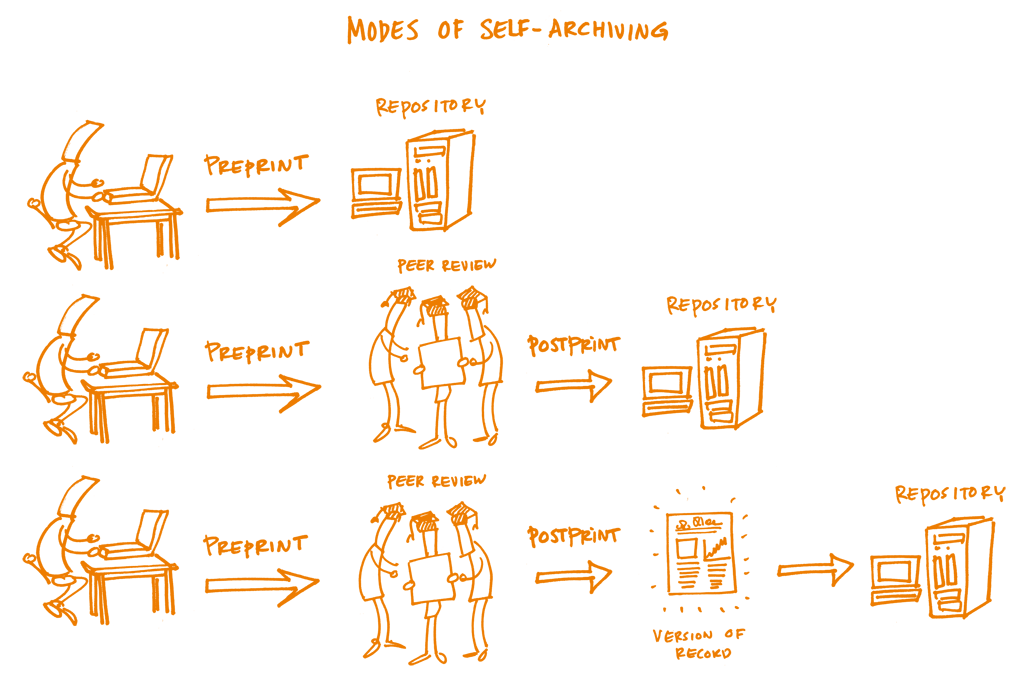
\includegraphics[width=0.8\textwidth]{hb_1.png}
\caption{Modes of self-archiving. Source: \citet{bezjak_open_2018}. License: \href{https://creativecommons.org/publicdomain/zero/1.0/deed.en}{CC0 1.0}.}
\end{figure}
\end{frame}

%------------------------------------------------------------------

\begin{frame}{Green OA: which version of a paper should you post online?}
	\begin{itemize}
    	\uncover<1->{
    	\item Each journal has its own self-archiving policy.
        }
        \uncover<2->{
        \item Find out about this policy \textbf{before} submitting your paper or uploading it on an online repository.
        }
        \uncover<3->{
        \item The best place to find out is \href{http://www.sherpa.ac.uk/romeo/index.php}{\textbf{SHERPA RoMEO}}, a database of journal self-archiving policies. 
        }
        \uncover<4->{
        \item SHERPA RoMEO uses a color code:
        }
        \begin{itemize}
        	\uncover<5->{
        	\item \textbf{\textcolor{green}{Green}} journals allow authors to archive pre and postprints.
            }
            \uncover<6->{
			\item \textbf{\textcolor{blue}{Blue}} journals allow authors to archive postprints.
            }
            \uncover<7->{
			\item \textbf{\textcolor{yellow}{Yellow}} journals allow authors to archive preprints.
            }
            \uncover<8->{
            \item White journals do not formally allow archiving.
            }
        \end{itemize}
        
	\end{itemize}
\end{frame}

%------------------------------------------------------------------

\begin{frame}{Green OA: green, blue, yellow, and white journals}
\begin{figure}
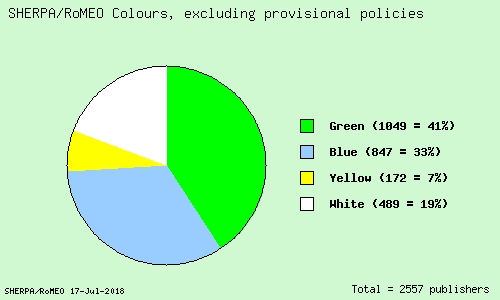
\includegraphics[width=0.8\textwidth]{sherpa.jpeg}
\caption{Share of green, blue, yellow, and white journals in the SHERPA RoMEO database. Source: \citet{sherpa_romeo_romeo_2018}. License: \href{https://creativecommons.org/licenses/by-nc-nd/2.0/uk/}{CC BY-NC-ND 2.0 UK}.}
\end{figure}
\end{frame}

%------------------------------------------------------------------

\begin{frame}{Green OA: more on preprints}
	\begin{itemize}
    	\uncover<1->{
    	\item Preprints allow authors to make early research findings available to the entire connected world for free.
        }
        \begin{enumerate}
        	\uncover<2->{
        	\item You upload a paper to a public repository.
            }
            \uncover<3->{
            \item The paper goes through a moderation process that assesses the scientific character of your work.
            }
            \uncover<4->{
            \item The paper is made available online. 
            }
        \end{enumerate}
        \uncover<5->{
        \item No wait, ``I won't be able to get published''
        }
        \begin{itemize}
        	\uncover<6->{
        	\item About \textbf{half} of all academic journals allow preprints.
            }
        \end{itemize}
        
        \uncover<7->{
        \item No wait, ``I will get scooped''
        }
        \begin{itemize}
        	\uncover<8->{
        	\item Preprints provide a \textbf{``record of priority''} \citep{bourne_ten_2017}.
            }
        \end{itemize}
	\end{itemize}
\end{frame}

%------------------------------------------------------------------

\begin{frame}{Green OA: where should you post your paper?}
	\begin{itemize}
    	\uncover<1->{
    	\item Three options
        }
        \begin{enumerate}
        	\uncover<2->{
        	\item On an institutional (university) repository
            \begin{itemize}
            	\item Example: \href{https://edoc.hu-berlin.de/}{HU's edoc-Server}
            \end{itemize}
            }
            \uncover<3->{
            \item On a thematic repository
            \begin{itemize}
            	\item Example: \href{https://socopen.org/}{SocArXiv}
            \end{itemize}
            }
            \uncover<4->{
            \item On a general repository
            \begin{itemize}
            	\item Example: \href{https://zenodo.org/}{Zenodo}
            \end{itemize}
            }
        \end{enumerate}
        \uncover<5->{
        \item A good repository:
        }
        \begin{itemize}
        	\uncover<6->{
        	\item has a sustainable server infrastructure,
            }
            \uncover<7->{
        	\item allows you to store supplementary material (code and data),
            }
            \uncover<8->{
            \item offers a permanent identifier (usually a DOI) for your project.
            }
        \end{itemize}
	\end{itemize}
\end{frame}

%------------------------------------------------------------------

\begin{frame}{}
\begin{figure}

\includegraphics[width=0.3\textwidth]{hb_2.png}
\end{figure}
\begin{center}
	\textbf{\large Small group discussion: pros and cons}
    
	Participants join small groups and discuss what are the advantages and disadvantages of different models of OA publishing: green, gold, and hybrid.

	We regroup in plenary to share our main conclusions.
\end{center}
\end{frame}

%------------------------------------------------------------------
% The State of OA
%------------------------------------------------------------------

\begin{frame}{}
\begin{center}
	\textbf{\large What is the share of open access publications in the scientific literature and what is their impact?}
\end{center}
\end{frame}

%------------------------------------------------------------------

\begin{frame}{A new push for OA}
	\begin{itemize}
    	\uncover<1->{
    	\item The share of OA papers has increased dramatically over the last 20 years.
        }
        \uncover<2->{
        \item This is driven by different factors:
        }
        \begin{enumerate}
        	\uncover<3->{
        	\item Funding institutions require projects to publish their results in OA.
            }
            \uncover<4->{
            \item OA publications are easily findable with tools like Google Scholar and the \textbf{Unpaywall} browser extension (highly recommended).
            }
            \uncover<5->{
            \item Academic social networks (ResearchGate and Academia.edu) are encouraging the diffusion of OA papers.
            }
            \uncover<6->{
            \item Universities are canceling subscriptions and looking to OA as an alternative \citep{piwowar_state_2018}.
            }
        \end{enumerate}
        \uncover<7->{
    	\item Best evidence of the growth of OA: Study by \citet{piwowar_state_2018}.
        }
	\end{itemize}
\end{frame}

%------------------------------------------------------------------

\begin{frame}{The prevalence of OA}
	\begin{figure}
		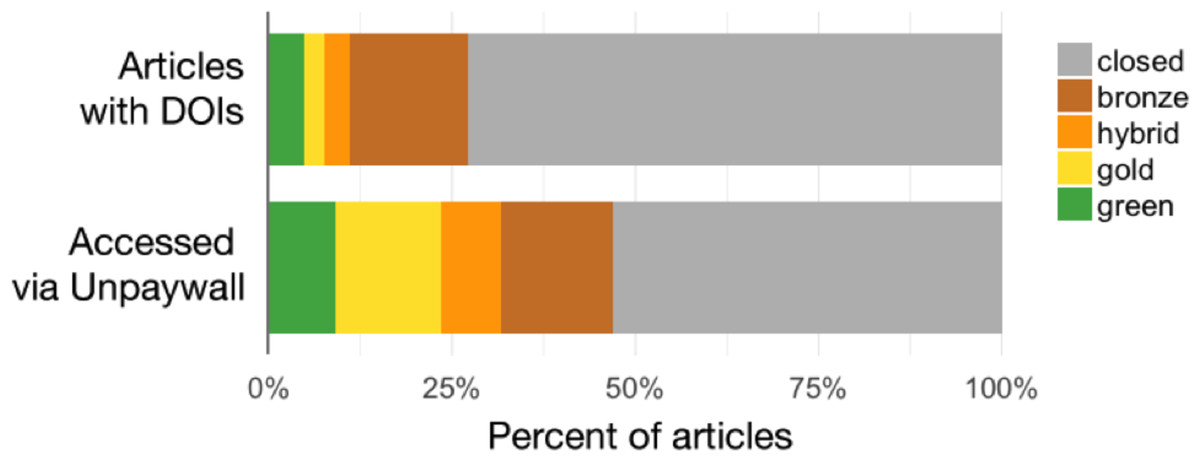
\includegraphics[width=\textwidth]{piwowar_et_al_1.jpg}
		\caption{Percent of articles by OA status, Crossref-DOIs sample vs Unpaywall-DOIs sample. Source: \citet{piwowar_state_2018}. License: \href{https://creativecommons.org/licenses/by/4.0/}{CC BY 4.0}.}
	\end{figure}
\end{frame}

%------------------------------------------------------------------

\begin{frame}{Growth over time}
	\begin{figure}
		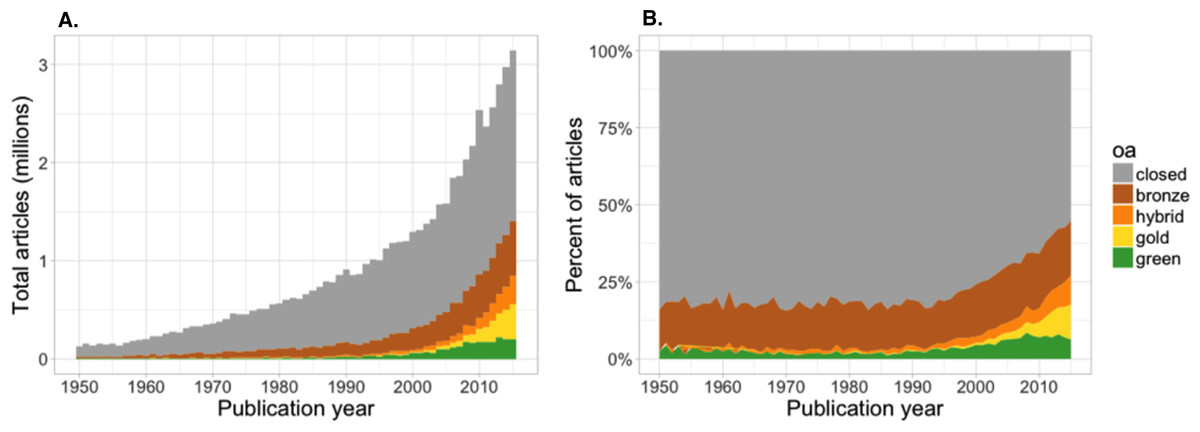
\includegraphics[width=\textwidth]{piwowar_et_al_2.jpg}
		\caption{Number of articles (A) and proportion of articles (B) with OA copies, estimated based on a random sample of 100,000 articles with Crossref DOIs. Source: \citet{piwowar_state_2018}. License: \href{https://creativecommons.org/licenses/by/4.0/}{CC BY 4.0}.}
	\end{figure}
\end{frame}

%------------------------------------------------------------------

\begin{frame}{Prevalence of OA by discipline}
	\begin{figure}
		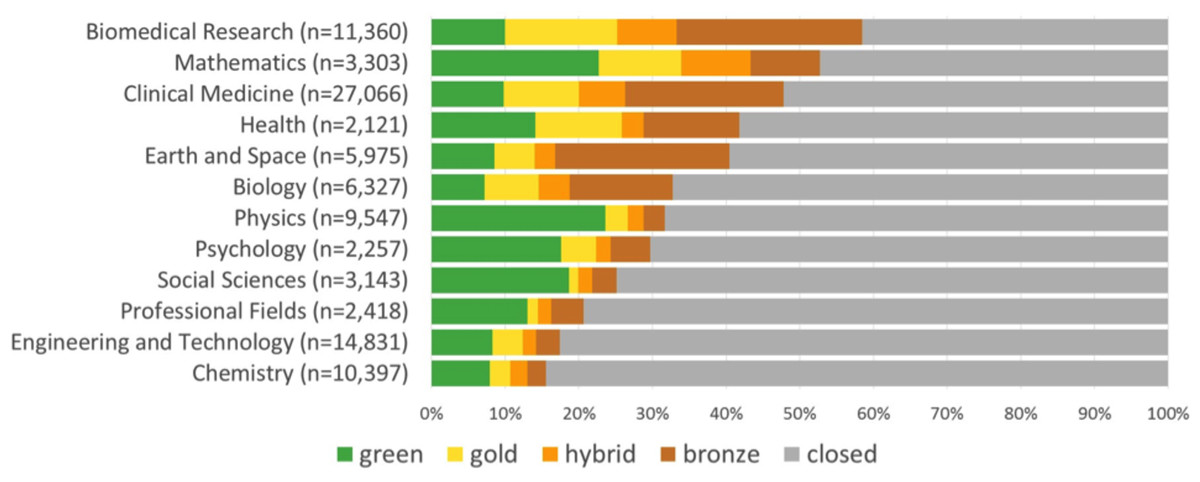
\includegraphics[width=\textwidth]{piwowar_et_al_3.jpg}
		\caption{Percentage of different access types of a random sample of WoS articles and reviews with a DOI published between 2009 and 2015 per NSF discipline (excluding Arts and Humanities). Source: \citet{piwowar_state_2018}. License: \href{https://creativecommons.org/licenses/by/4.0/}{CC BY 4.0}.}
	\end{figure}
\end{frame}

%------------------------------------------------------------------

\begin{frame}{The impact of OA publications}
	\begin{figure}
		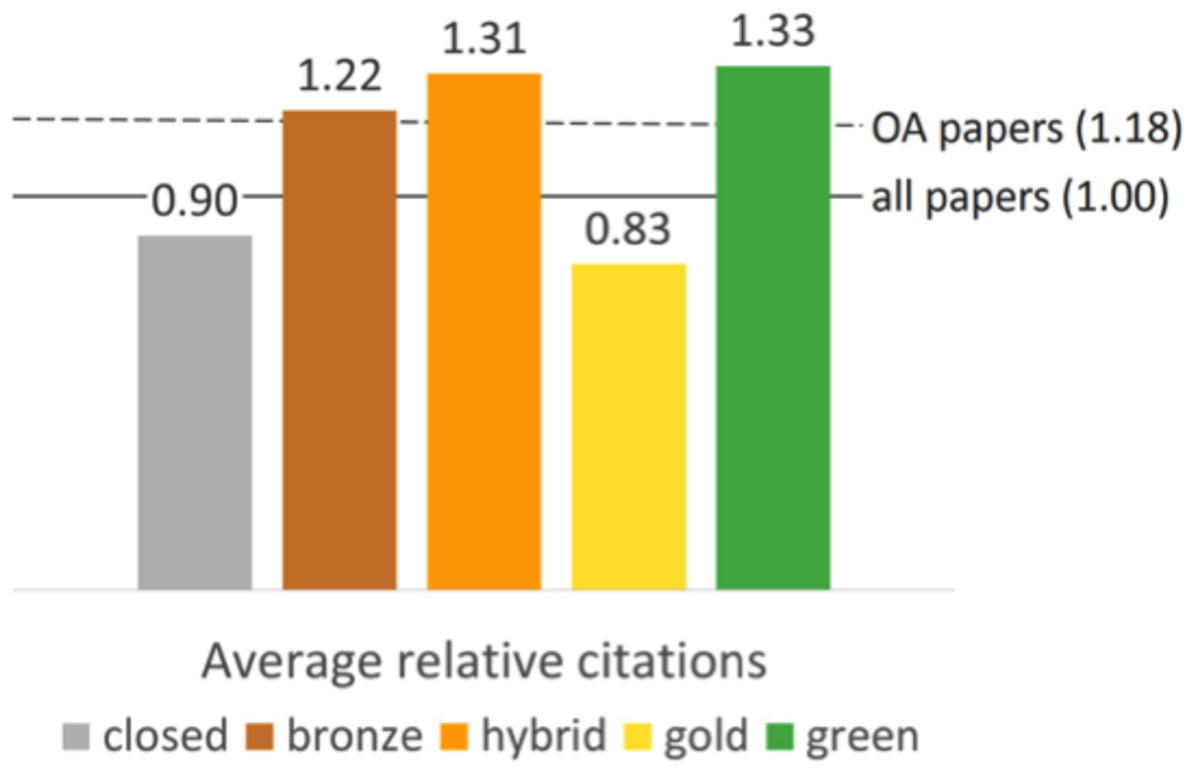
\includegraphics[width=0.8\textwidth]{piwowar_et_al_4.jpg}
		\caption{Average relative citations of different access types of a random sample of WoS articles and reviews with a DOI published between 2009 and 2015.). License: \href{https://creativecommons.org/licenses/by/4.0/}{CC BY 4.0}.}
	\end{figure}
\end{frame}

%------------------------------------------------------------------
% Licenses
%------------------------------------------------------------------

\begin{frame}{}
\begin{center}
	\textbf{\large Which license should you choose?}
\end{center}
\end{frame}

%------------------------------------------------------------------

\begin{frame}{The Creative Commons Licenses}
	\begin{itemize}
    	\uncover<1->{
    	\item Creative Commons are the default option.
        }
        \uncover<2->{
        \item All CC licenses help authors \textbf{retain their copyright} while allowing others to make use of their work under certain conditions.
        }
	\end{itemize}
\end{frame}

%------------------------------------------------------------------

\begin{frame}{CC-BY}
	\begin{figure}
		\includegraphics[width=0.25\textwidth]{ccby.eps}
		\caption{CC-BY. Source: \citet{creative_commons_about_2018}  License: \href{https://creativecommons.org/licenses/by/4.0/}{CC BY 4.0}.}
	\end{figure}
	\begin{itemize}
    	\uncover<1->{
    	\item The \textbf{least restrictive} of all CC licenses.
        }
        \begin{itemize}
        	\uncover<2->{
        	\item ``This license lets others distribute, remix, tweak, and build upon your work, even commercially, as long as they credit you for the original creation'' \citep{creative_commons_about_2018}. 
            }
        \end{itemize}
        \uncover<3->{
        \item CC-BY has become the \textbf{gold standard} in OA publishing as it maximizes the dissemination of research findings \citep{redhead_why_2012,kreutzer_open_2014}. 
        }
	\end{itemize}
\end{frame}

%------------------------------------------------------------------

\begin{frame}{Variants of CC-BY}
	\begin{enumerate}
    	\uncover<1->{
    	\item CC-BY-NC: Attribution-NonCommercial
        }
        \uncover<2->{
        \item CC-BY-ND: Attribution-NoDerivs
        }
        \uncover<3->{
        \item CC-BY-SA: Attribution-ShareAlike
        }
        \uncover<4->{
        \item CC-BY-NC-ND
        }
        \uncover<5->{
        \item CC-BY-NC-SA
        }
	\end{enumerate}
\end{frame}

%------------------------------------------------------------------

\begin{frame}{A spectrum of restrictions}
	\begin{figure}
		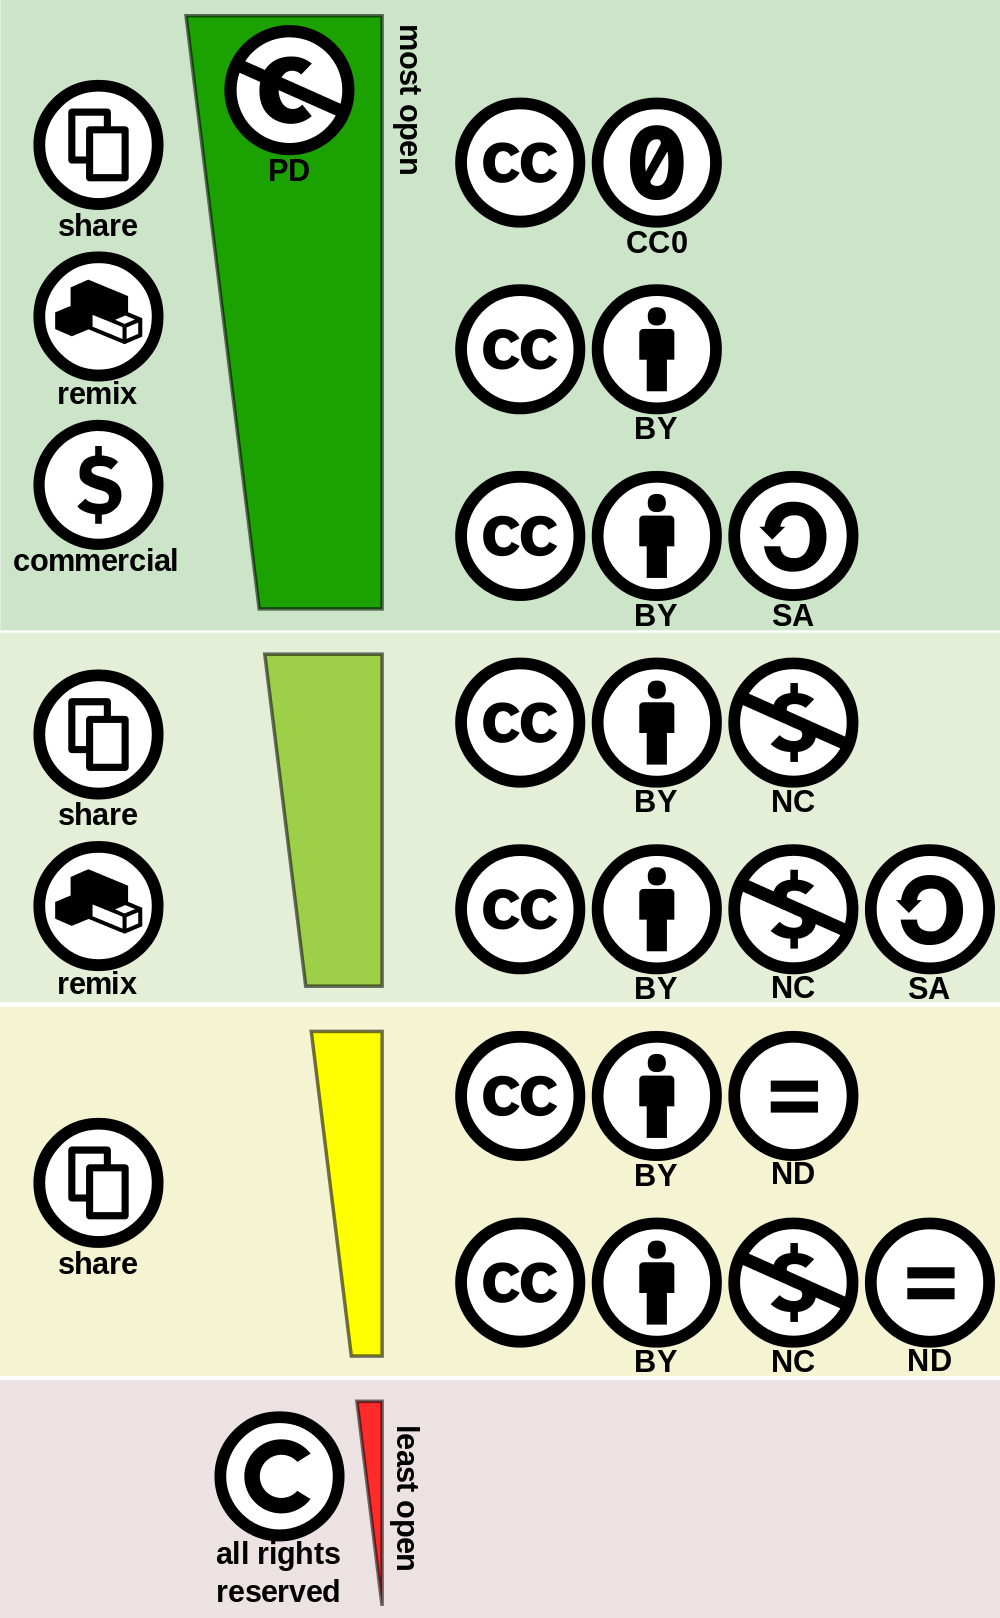
\includegraphics[width=0.35\textwidth]{cc_spectrum.png}
		\caption{CC license spectrum between public domain (top) and all rights reserved (bottom). Source: \citet{shaddim_file:creative_2016}  License: \href{https://creativecommons.org/licenses/by/4.0/}{CC BY 4.0}.}
	\end{figure}
\end{frame}

%------------------------------------------------------------------
% Licenses
%------------------------------------------------------------------

\begin{frame}{}
\begin{center}
	\textbf{\large How to find funding for your open access publication?}
\end{center}
\end{frame}


%------------------------------------------------------------------

\begin{frame}{Funding options}
	\begin{itemize}
    	\uncover<1->{
    	\item Do you need to pay APCs?
        }
        \begin{itemize}
        	\uncover<2->{
        	\item 70\% of OA journals are free.
            }
            \uncover<3->{
            \item Have you thought about self-archiving (green OA)?
            }
        \end{itemize}
        \uncover<4->{
        \item If you need to pay APCs
        }
        \begin{enumerate}
        	\uncover<5->{
        	\item If you are in a project, look if your funder has an OA publication fund.
            }
            \uncover<6->{
            \item Look if your university, faculty, or department has an OA publication fund.
            }
            \uncover<7->{
            \item Ask your supervisor if there is internal funding available.
            }
            \uncover<8->{
            \item Look if you are admissible for a waiver (lower income countries). 
            }
        \end{enumerate}
	\end{itemize}
\end{frame}

%------------------------------------------------------------------
% Practical examples
%------------------------------------------------------------------

\begin{frame}{}
\begin{figure}

\includegraphics[width=0.3\textwidth]{hb_2.png}
\end{figure}
\begin{center}
	\textbf{\large Practical examples}
\end{center}
\end{frame}

%------------------------------------------------------------------

\begin{frame}{Find a self-archiving policy on SHERPA RoMEO}
	\begin{itemize}
    	\item Question 1
        \begin{itemize}
    		\item Go to http://www.sherpa.ac.uk/romeo
        	\item Look for the self-archiving policy of the \textit{European Sociological Review}
            \item Which color code was given to the journal and what rights does it grant authors?
		\end{itemize}
        \item Question 2
        \begin{itemize}
    		\item Go to http://www.sherpa.ac.uk/romeo
        	\item Look for the self-archiving policy of the \textit{European Journal of Political Research}
            \item Which color code was given to the journal and what rights does it grant authors?
		\end{itemize}
	\end{itemize}
\end{frame}


%------------------------------------------------------------------

\begin{frame}{Find a gold OA journal on the Directory of Open Access Journals (DOAJ)}
	\begin{itemize}
    	\item Question 3
        \begin{itemize}
    		\item Go to https://doaj.org
        	\item Click ``Search'' in the top menu
            \item Look for: 
            \begin{itemize}
    			\item \textbf{journals}
        		\item with \textbf{Social Sciences} as subject
            	\item with \textbf{no APCs}
                \item with a \textbf{CC-BY} license
                \item where the full text is in \textbf{English}
                \item and peer review is \textbf{double-blind}
		\end{itemize}
        \item How many journals can you find?
		\end{itemize}
	\end{itemize}
\end{frame}


%------------------------------------------------------------------

\begin{frame}{Look for a preprint on SocArXiv}
	\begin{itemize}
    \item Question 4
      \begin{itemize}
          \item Go to http://socarxiv.org
          \item Search a paper on ``Protest in Eastern Germany'', last edited in July 2018.
          \item Click on the title
          \item Scroll down the preprint page and click on ``Visit project'' 
          \item What additional components are made available by the author?
      \end{itemize}
    \end{itemize}
\end{frame}

%------------------------------------------------------------------

\begin{frame}{}
\begin{center}
	\textbf{\large Thank you!}
\end{center}
\end{frame}

%------------------------------------------------------------------
% References
%------------------------------------------------------------------
\appendix
\begin{frame}[allowframebreaks]{References}
\bibliographystyle{apacite}
\bibliography{bibliography.bib}
\end{frame}

%------------------------------------------------------------------
\end{document}
